\documentclass[tikz,border=8pt]{standalone}
\usetikzlibrary{shapes.geometric, arrows.meta, positioning, fit, backgrounds, calc, matrix}

% ---------- colours ----------
\definecolor{cIO}{HTML}{AED6F1}    % input / output / permute
\definecolor{cConv}{HTML}{FAD7A0}  % conv layers
\definecolor{cNorm}{HTML}{A9DFBF}  % norm + activation (+ dropout)
\definecolor{cGRU}{HTML}{D2B4DE}   % GRUBlock outer
\definecolor{cInt}{HTML}{F2F3F4}   % GRUBlock / AttentionPool internals
\definecolor{cAtt}{HTML}{FCF3CF}   % AttentionPool
\definecolor{cHead}{HTML}{FADBD8}  % classification head

\pgfdeclarelayer{background}
\pgfsetlayers{background,main}

\tikzset{
  bx/.style={draw, rounded corners=2pt, minimum height=0.55cm,
             align=center, font=\scriptsize, inner sep=2pt},
  io/.style={bx, fill=cIO, minimum height=0.7cm},
  cv/.style={bx, fill=cConv, minimum width=4.6cm, minimum height=0.55cm},
  nm/.style={bx, fill=cNorm, minimum width=4.6cm},
  gb/.style={bx, fill=cGRU, minimum width=2.7cm, minimum height=0.9cm},
  attn/.style={bx, fill=cAtt, minimum width=2.8cm, minimum height=0.9cm},
  hd/.style={bx, fill=cHead, minimum width=1.7cm, minimum height=0.7cm},
  inn/.style={bx, fill=cInt, minimum width=4.0cm, minimum height=0.5cm},
  arr/.style={-{Stealth[length=1.8mm,width=1.5mm]}, thick},
  lbl/.style={font=\tiny\ttfamily, inner sep=1pt},
  fbox/.style={draw, rounded corners=4pt, inner sep=5pt},
  ttl/.style={font=\scriptsize\bfseries, inner sep=1.5pt},
  sw/.style={draw, minimum size=3mm, inner sep=0pt},
}

% arrows with tensor-shape labels:  \hh = horizontal (label above)
%                                   \vr = vertical (label right)
%                                   \vl = vertical (label left)
\newcommand{\hh}[3]{\draw[arr] (#1) -- node[lbl,above=1pt]{#3} (#2);}
\newcommand{\vr}[3]{\draw[arr] (#1) -- node[lbl,right=1.5pt]{#3} (#2);}
\newcommand{\vl}[3]{\draw[arr] (#1) -- node[lbl,left=1.5pt]{#3} (#2);}

\begin{document}
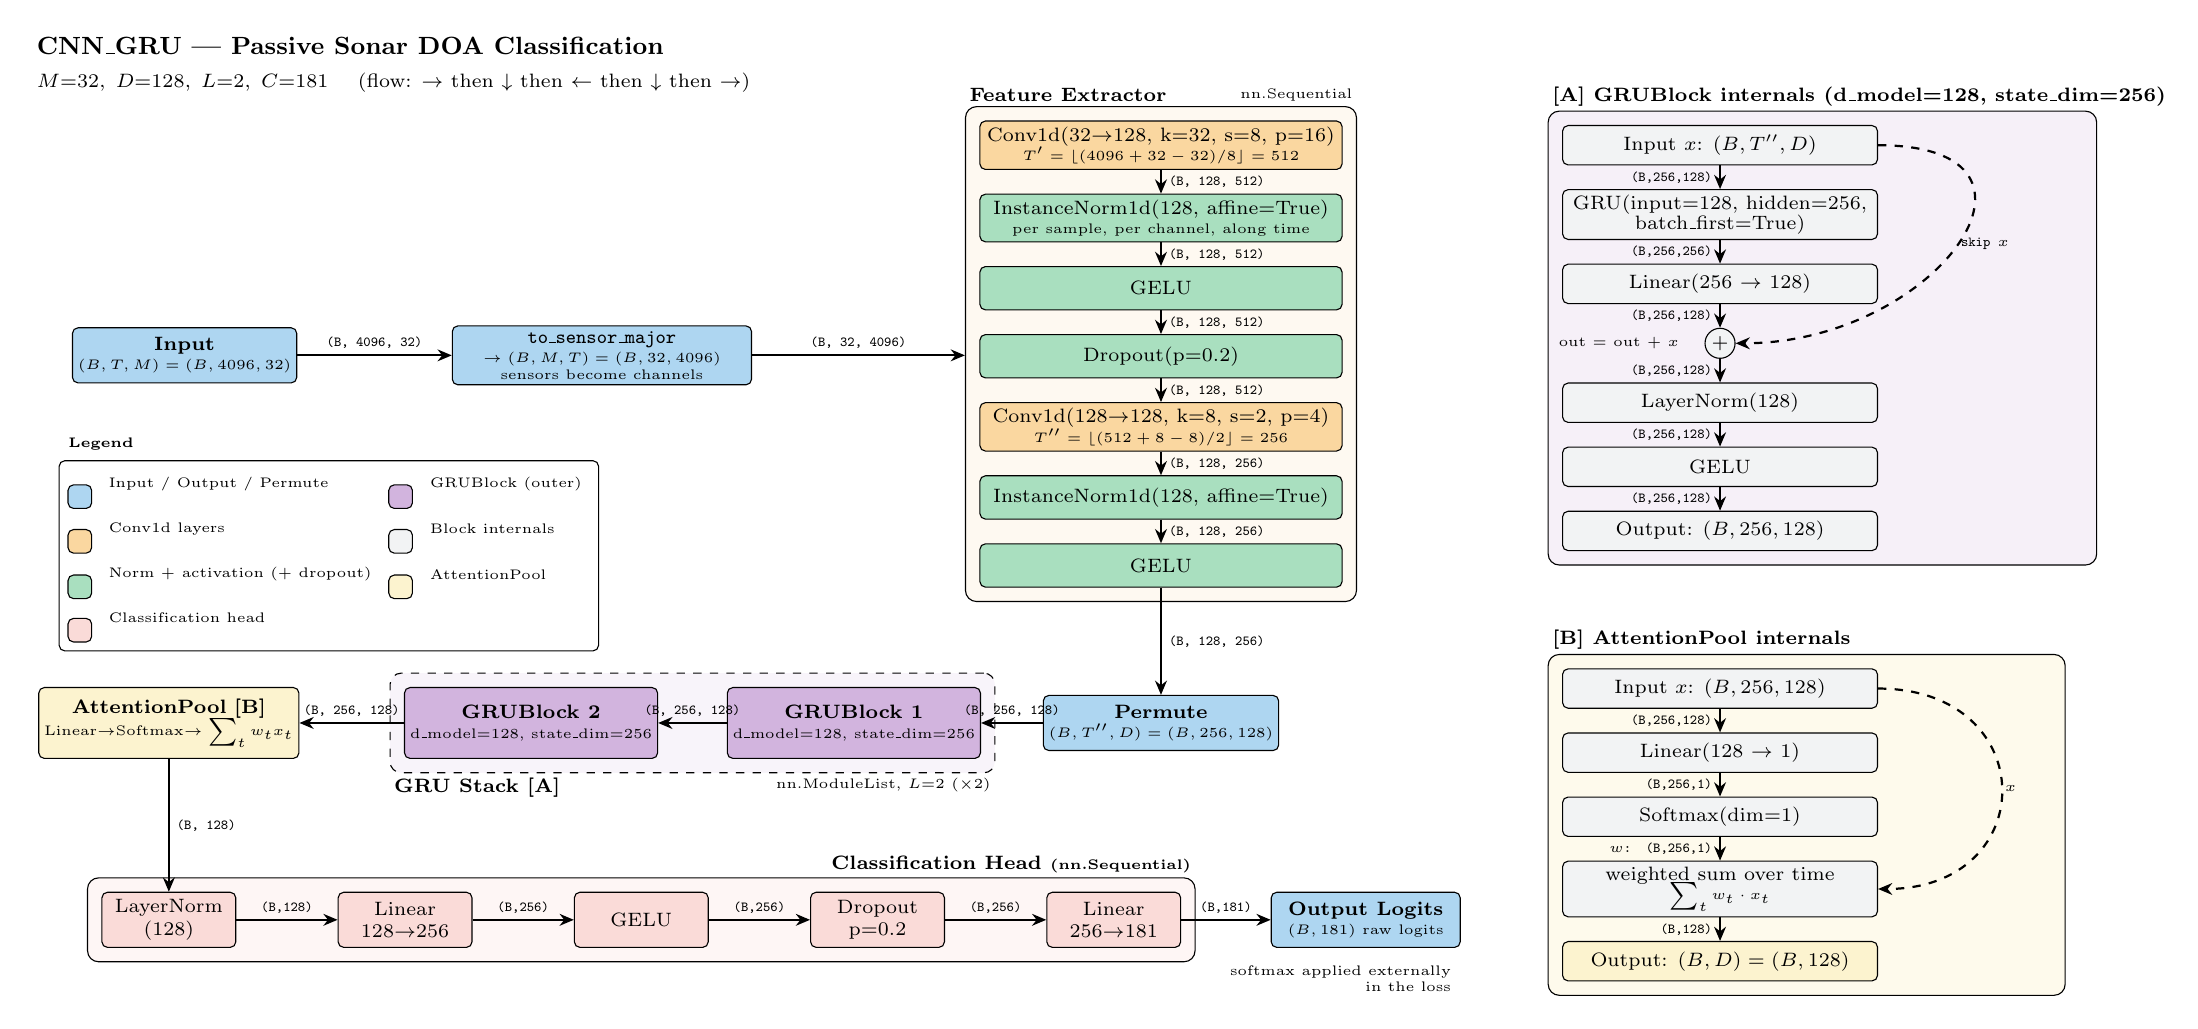
\begin{tikzpicture}[node distance=3mm]

%=====================================================================
% ROW 1  (left -> right):  Input -> to_sensor_major -> Feature Extractor
%=====================================================================
\node[cv] (c1) at (14,0)
  {Conv1d(32$\to$128, k=32, s=8, p=16)\\[-1pt]
   {\tiny $T'=\lfloor(4096+32-32)/8\rfloor=512$}};
\node[nm, below=of c1] (n1)
  {InstanceNorm1d(128, affine=True)\\[-1pt]
   {\tiny per sample, per channel, along time}};
\node[nm, below=of n1] (g1) {GELU};
\node[nm, below=of g1] (d1) {Dropout(p=0.2)};
\node[cv, below=of d1] (c2)
  {Conv1d(128$\to$128, k=8, s=2, p=4)\\[-1pt]
   {\tiny $T''=\lfloor(512+8-8)/2\rfloor=256$}};
\node[nm, below=of c2] (n2) {InstanceNorm1d(128, affine=True)};
\node[nm, below=of n2] (g2) {GELU};

\coordinate (fec) at ($(c1)!0.5!(g2)$);   % vertical centre of the extractor

\node[io, minimum width=2.8cm] (inp) at ($(fec)+(-12.4,0)$)
  {\textbf{Input}\\[-1pt]{\tiny $(B,T,M)=(B,4096,32)$}};
\node[io, minimum width=3.8cm] (perm1) at ($(fec)+(-7.1,0)$)
  {\texttt{to\_sensor\_major}\\[-1pt]
   {\tiny $\to (B,M,T)=(B,32,4096)$}\\[-2pt]
   {\tiny sensors become channels}};

% arrows inside the extractor
\vr{c1}{n1}{(B, 128, 512)}
\vr{n1}{g1}{(B, 128, 512)}
\vr{g1}{d1}{(B, 128, 512)}
\vr{d1}{c2}{(B, 128, 512)}
\vr{c2}{n2}{(B, 128, 256)}
\vr{n2}{g2}{(B, 128, 256)}

%=====================================================================
% ROW 2  (right -> left):  Permute -> GRUBlock 1 -> GRUBlock 2 -> AttentionPool
%=====================================================================
\node[io, minimum width=2.4cm] (perm2) at ($(g2)+(0,-2.0)$)
  {\textbf{Permute}\\[-1pt]{\tiny $(B,T'',D)=(B,256,128)$}};
\node[gb] (gb1) at ($(perm2)+(-3.9,0)$)
  {\textbf{GRUBlock 1}\\[-1pt]{\tiny d\_model=128, state\_dim=256}};
\node[gb] (gb2) at ($(perm2)+(-8.0,0)$)
  {\textbf{GRUBlock 2}\\[-1pt]{\tiny d\_model=128, state\_dim=256}};
\node[attn] (ap) at ($(perm2)+(-12.6,0)$)
  {\textbf{AttentionPool} \textbf{[B]}\\[-1pt]
   {\tiny Linear$\to$Softmax$\to\sum_t w_t x_t$}};

\vr{g2}{perm2}{(B, 128, 256)}
\hh{perm2.west}{gb1.east}{(B, 256, 128)}
\hh{gb1.west}{gb2.east}{(B, 256, 128)}
\hh{gb2.west}{ap.east}{(B, 256, 128)}

%=====================================================================
% ROW 3  (left -> right):  Classification Head -> Output
%=====================================================================
\node[hd] (h1) at ($(perm2)+(-12.6,-2.5)$) {LayerNorm\\(128)};
\node[hd] (h2) at ($(perm2)+(-9.6,-2.5)$)  {Linear\\128$\to$256};
\node[hd] (h3) at ($(perm2)+(-6.6,-2.5)$)  {GELU};
\node[hd] (h4) at ($(perm2)+(-3.6,-2.5)$)  {Dropout\\p=0.2};
\node[hd] (h5) at ($(perm2)+(-0.6,-2.5)$)  {Linear\\256$\to$181};
\node[io, minimum width=2.4cm] (out) at ($(perm2)+(2.6,-2.5)$)
  {\textbf{Output Logits}\\[-1pt]{\tiny $(B,181)$ raw logits}};

\vr{ap}{h1}{(B, 128)}
\hh{h1.east}{h2.west}{(B,128)}
\hh{h2.east}{h3.west}{(B,256)}
\hh{h3.east}{h4.west}{(B,256)}
\hh{h4.east}{h5.west}{(B,256)}
\hh{h5.east}{out.west}{(B,181)}
\node[font=\tiny, anchor=north east, align=right] at ($(out.south east)+(0,-1mm)$)
  {softmax applied externally\\in the loss};

%=====================================================================
% DETAIL [A]: GRUBlock internals (right column, top)
%=====================================================================
\node[inn] (g_in) at ($(c1)+(7.1,0)$) {Input $x$: $(B,T'',D)$};
\node[inn, below=of g_in] (g_gru)
  {GRU(input=128, hidden=256,\\[-1pt]batch\_first=True)};
\node[inn, below=of g_gru] (g_lin) {Linear(256 $\to$ 128)};
\node[circle, draw, fill=cInt, inner sep=1pt, font=\scriptsize, below=of g_lin] (g_add) {$+$};
\node[left=2mm of g_add, font=\tiny, anchor=east] {out = out + $x$};
\node[inn, below=of g_add] (g_ln) {LayerNorm(128)};
\node[inn, below=of g_ln] (g_ge) {GELU};
\node[inn, below=of g_ge] (g_out) {Output: $(B,256,128)$};

\vl{g_in}{g_gru}{(B,256,128)}
\vl{g_gru}{g_lin}{(B,256,256)}
\vl{g_lin}{g_add}{(B,256,128)}
\vl{g_add}{g_ln}{(B,256,128)}
\vl{g_ln}{g_ge}{(B,256,128)}
\vl{g_ge}{g_out}{(B,256,128)}

% curved residual skip around GRU -> Linear
\draw[arr, dashed, thick] (g_in.east) to[out=0,in=0,looseness=2.1]
  node[lbl, right, pos=0.5]{skip $x$} (g_add.east);
\coordinate (gskip) at ($(g_in.east)+(2.6,0)$);

%=====================================================================
% DETAIL [B]: AttentionPool internals (right column, bottom)
%=====================================================================
\node[inn] (a_in) at ($(g_in)+(0,-6.9)$) {Input $x$: $(B,256,128)$};
\node[inn, below=of a_in] (a_lin) {Linear(128 $\to$ 1)};
\node[inn, below=of a_lin] (a_sm) {Softmax(dim=1)};
\node[inn, below=of a_sm] (a_sum)
  {weighted sum over time\\[-1pt]{\tiny $\sum_t w_t\cdot x_t$}};
\node[inn, fill=cAtt, below=of a_sum] (a_out) {Output: $(B,D)=(B,128)$};

\vl{a_in}{a_lin}{(B,256,128)}
\vl{a_lin}{a_sm}{(B,256,1)}
\vl{a_sm}{a_sum}{$w$: (B,256,1)}
\vl{a_sum}{a_out}{(B,128)}
\draw[arr, dashed, thick] (a_in.east) to[out=0,in=0,looseness=2.1]
  node[lbl, right, pos=0.5]{$x$} (a_sum.east);
\coordinate (askip) at ($(a_in.east)+(2.2,0)$);

%=====================================================================
% FRAMES (background layer)
%=====================================================================
\begin{pgfonlayer}{background}
  \node[fbox, fill=cConv!15, fit=(c1)(g2),
        label={[ttl, anchor=south west]north west:Feature Extractor},
        label={[ttl, font=\tiny, anchor=south east]north east:nn.Sequential}] (fe) {};

  \node[fbox, dashed, fill=cGRU!15, fit=(gb1)(gb2),
        label={[ttl, anchor=north west]south west:GRU Stack \textbf{[A]}},
        label={[ttl, font=\tiny, anchor=north east]south east:nn.ModuleList, $L{=}2$ ($\times 2$)}] (stk) {};

  \node[fbox, fill=cHead!25, fit=(h1)(h5),
        label={[ttl, anchor=south east]north east:Classification Head {\tiny (nn.Sequential)}}] (hdf) {};

  \node[fbox, fill=cGRU!20, fit=(g_in)(g_out)(gskip),
        label={[ttl, anchor=south west]north west:[A] GRUBlock internals (d\_model=128, state\_dim=256)}] (gfr) {};

  \node[fbox, fill=cAtt!40, fit=(a_in)(a_out)(askip),
        label={[ttl, anchor=south west]north west:[B] AttentionPool internals}] (afr) {};
\end{pgfonlayer}

% arrow from permute node into the Feature Extractor frame
\draw[arr] (perm1.east) -- node[lbl,above=1pt]{(B, 32, 4096)} (fe.west |- perm1);
\hh{inp.east}{perm1.west}{(B, 4096, 32)}

%=====================================================================
% TITLE + LEGEND
%=====================================================================
\node[anchor=north west, align=left, font=\small\bfseries] at (-0.4,1.5)
  {CNN\_GRU --- Passive Sonar DOA Classification\\[1pt]
   {\scriptsize\mdseries $M{=}32,\; D{=}128,\; L{=}2,\; C{=}181$ \quad
    (flow: $\rightarrow$ then $\downarrow$ then $\leftarrow$ then $\downarrow$ then $\rightarrow$)}};

\matrix[draw, rounded corners=2pt, fill=white, font=\tiny, inner sep=3pt,
        row sep=2pt, column sep=3pt, anchor=north west, ampersand replacement=\&]
  (leg) at (0,-4.0) {
  \node[sw, fill=cIO]{};   \& \node[anchor=west]{Input / Output / Permute};
  \& \node[sw, fill=cGRU]{}; \& \node[anchor=west]{GRUBlock (outer)};\\
  \node[sw, fill=cConv]{}; \& \node[anchor=west]{Conv1d layers};
  \& \node[sw, fill=cInt]{}; \& \node[anchor=west]{Block internals};\\
  \node[sw, fill=cNorm]{}; \& \node[anchor=west]{Norm + activation (+ dropout)};
  \& \node[sw, fill=cAtt]{}; \& \node[anchor=west]{AttentionPool};\\
  \node[sw, fill=cHead]{}; \& \node[anchor=west]{Classification head}; \& \& \\
};
\node[font=\tiny\bfseries, anchor=south west] at (leg.north west) {Legend};

\end{tikzpicture}
\end{document}
